% !TeX root = ../main.tex
% Add the above to each chapter to make compiling the PDF easier in some editors.

\chapter{INTRODUCTION}\label{chapter:introduction}

It is safe to say that the internet paved the way for many things for humanity.
Media such as images, video and audio can be shared across websites and applications, knowledge can be stored on faraway servers.
This knowledge can then be retrieved with ease in text format using mobile devices, and products and services can be bought with the click of a button or a tap on a screen.
Interactions, media and information make up for massive amounts of data that flow through complex computer systems, which in turn generate even more data and information.

Researchers have found ways to leverage the magnitude of data that is being produced every second by countless systems all around the world.
One of the most recent and most popular uses of this huge variety and quantity of data is machine learning (ML).
Machine learning can be defined as a set of techniques that use data to improve performance in a set of tasks.
Today, for example, we feed data to machine learning models to calculate what is the probability that a webpage visitor will buy certain products, or the chances that it is going to rain in a few days or to generate elaborate text and stunning, never-before-seen pictures.

Recently, models such as BERT \cite{devlin2018bert}, DALL-E \cite{ramesh2021zero}, GPT-3 \cite{brown2020gpt3} and others have become incredibly popular thanks to their outstanding results and endless possibilities.
DALL-E for example can generate high-quality realistic images and art starting from a text description written in natural language.
These models however require massive amounts of data as well as very expensive computational resources, such as graphical processing units and tensor processing units (TPUs).
In recent years, the size of neural network models has been steadily increasing exponentially, as shown by \autoref{fig:model-size-over-time}.
A simple calculation shows that the neural network model Megatron-Turing-NLG 530B \cite{smith2022megatronturingnlg} would take roughly $530 \times 4 = 2120\texttt{GB}$ of memory to simply hold its 530 billion weights.

Furthermore, training a neural network model requires even more memory.
Intermediate computation outputs such as gradient and optimizer states sometimes require 2 or 3 times as much memory than just the model parameters, making GPU memory one of the main bottlenecks in training huge neural network models.
While some of these issues can be tackled using techniques such as parameter quantization \cite{DBLP:journals/corr/abs-2003-11316}, pruning and compression, they must not be considered one-fits-all solutions.
Some models are simply too big to be trained on a single device.
This problem is exacerbated by factors such as high GPU prices and much slower growth of their memory size relative to model size.
\autoref{fig:gpu-vram-over-time} shows how GPU memory has been increasing from 2016 to 2022.

\begin{figure}[h]
    \caption{GPU VRAM over the past 4 years. The growth is mostly linear, doubling }
    \label{fig:gpu-vram-over-time}
    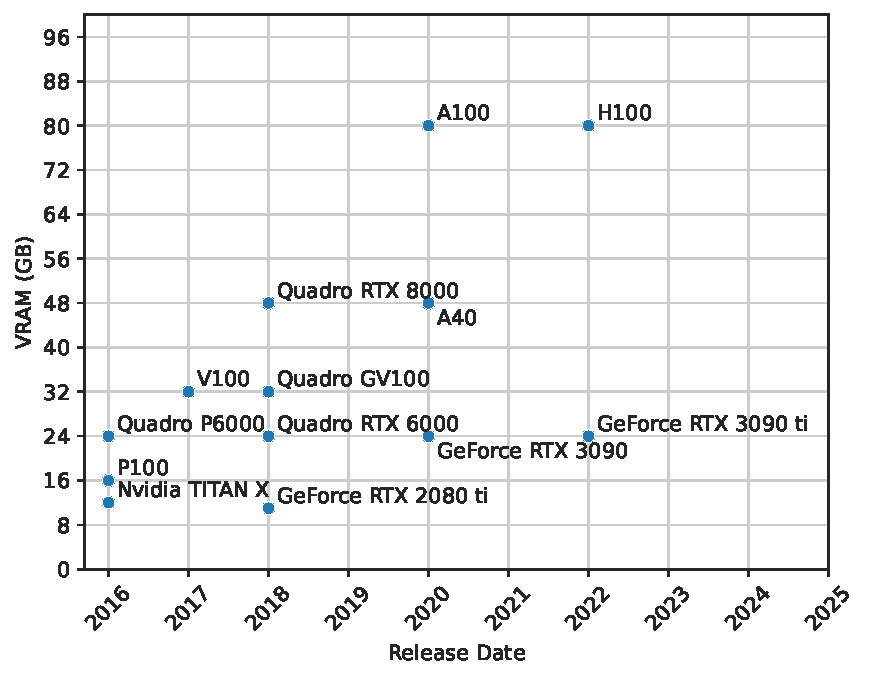
\includegraphics[width=\textwidth]{./figures/gpu-vram-over-time.pdf}
\end{figure}

\begin{figure}[h]
    \caption{Model size over the past 4 years: ELMo \cite{peters2018elmo}, BERT \cite{devlin2018bert}, GPT-2 \cite{radford2019language}, Megatron-LM \cite{shoeybi2019megatronlm}, T-5 \cite{raffael2019t5}, Turing-NLG \cite{microsoft2020turingnlg}, GPT-3 \cite{brown2020gpt3}, Megatron-Turing-NLG \cite{smith2022megatronturingnlg}}
    \label{fig:model-size-over-time}
    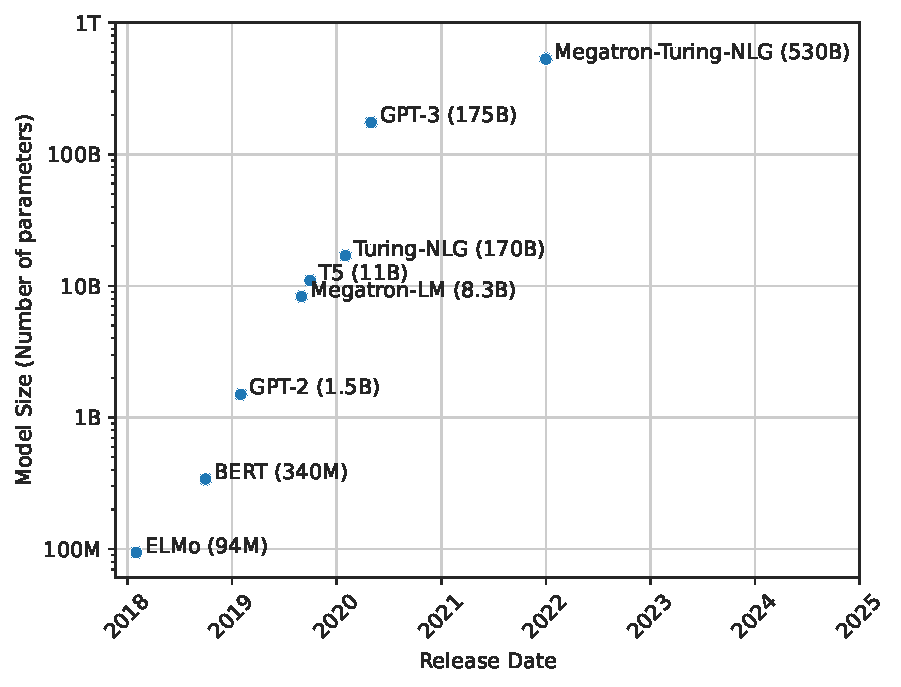
\includegraphics[width=\textwidth]{./figures/model-size-over-time.pdf}
\end{figure}

The characteristics of the latest GPU released by NVIDIA earlier in 2022, the H100 with 80GB of memory, an amount that hasn't changed since its direct predecessor A100.

To tackle this problem, practitioners studied and developed distributed computing techniques to train models that do not fit entirely in a single GPU's memory, distributing the training load to potentially thousands of devices.
One of the first, most prominent examples of distributed parallelism is the AlexNet network \cite{alexnet2012}, summarized in \autoref{fig:alexnet}.

\begin{figure}[h]
    \caption{AlexNet \cite{alexnet2012} architecture shows one of the first examples of model parallelism. The training of convolutional layers is split across two GPUs, as the size of the model during training exceeded the available memory of a single GPU.}
    \label{fig:alexnet}
    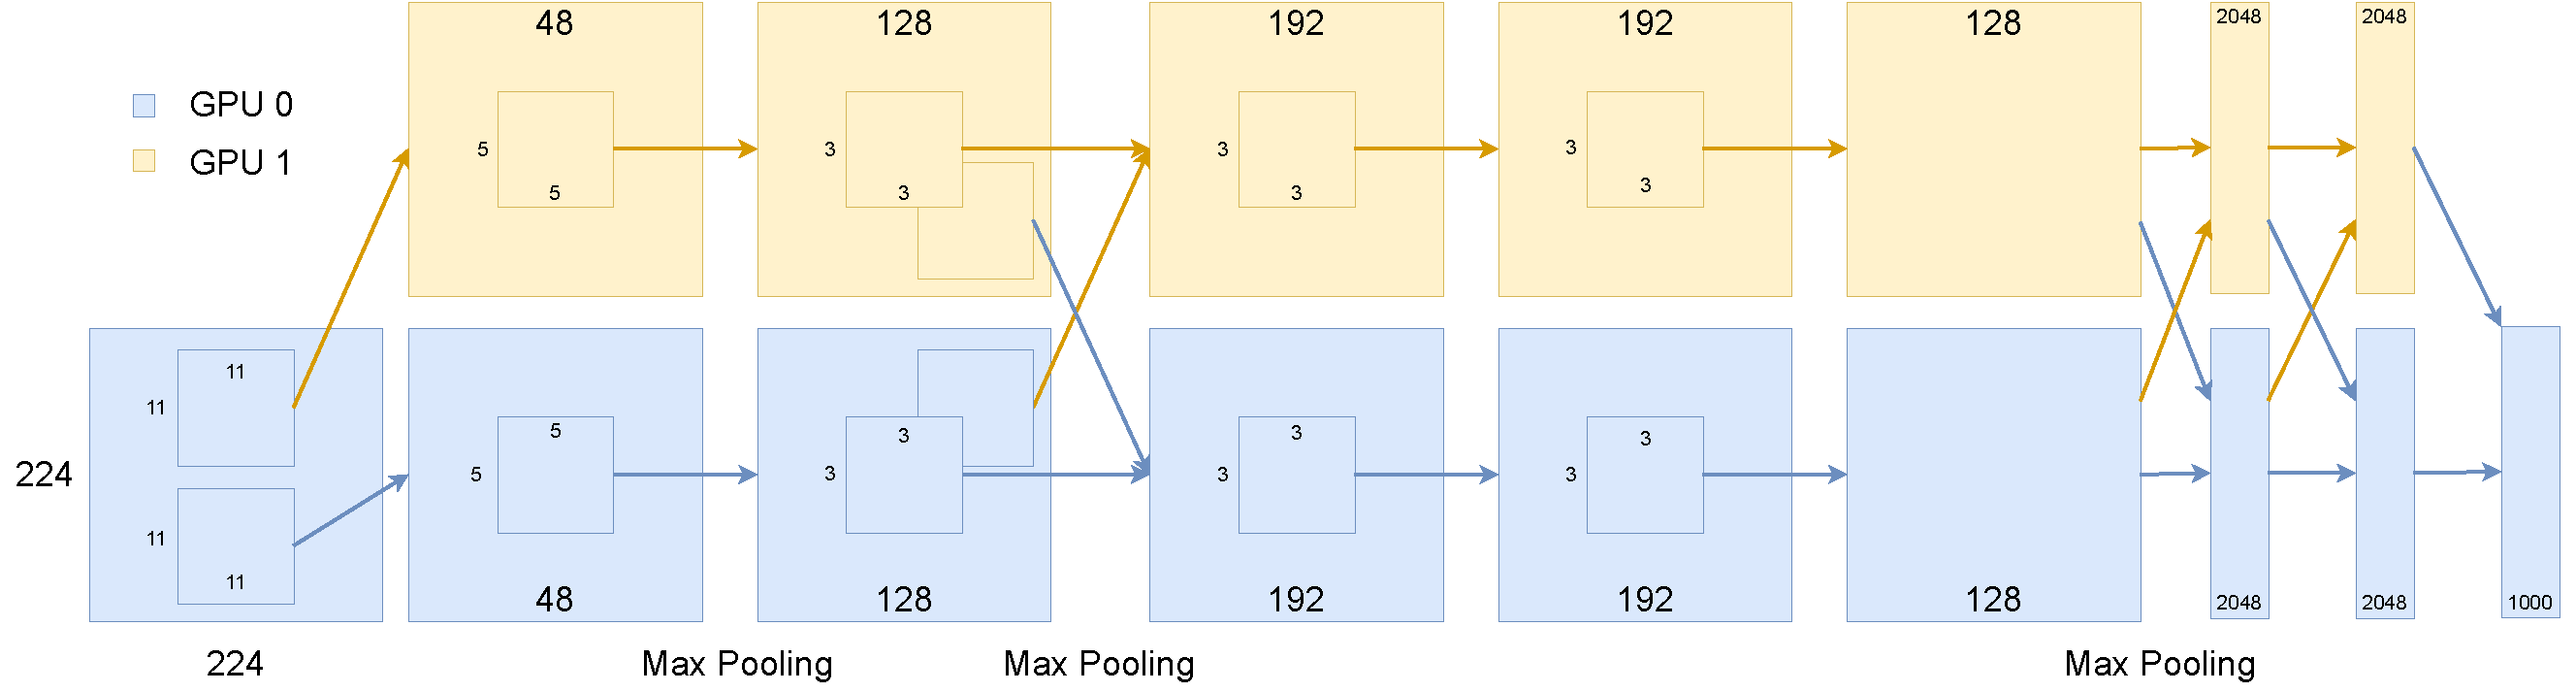
\includegraphics[width=\textwidth]{./figures/alexnet.pdf}
\end{figure}

Since then, the area of distributed training for neural networks has expanded, eventually leading to the creation of Hivemind.
Most of the frameworks and papers built on top of the techniques presented previously approach scalability issues by employing tremendous amounts of expensive, top-of-the-art and homogeneous hardware.
However, universities, small companies and hobbyists that want to train the models described in these papers do not necessarily have access to a such vast amount of resources, limiting possibilities and research directions.

The framework Hivemind \cite{riabinin2020hivemind} aims to help with these issues by allowing distributed neural network training across the internet using heterogeneous devices.
The authors provide two types of training: \textit{decentralized parameter averaging} and \textit{decentralized mixture-of-experts}.

Hivemind implements two training algorithms: ``Decentralized Mixture-of-Experts'' (DMoE) \cite{ryabinin2020learning} and ``Parameter Averaging''.
In this thesis, we will focus our efforts on decentralized parameter averaging.
With this technique, every node participating in a Hivemind training network must have a copy of the model in its local memory.
Each node performs training at its own pace, processing samples toward a global goal called ``target batch size''.
Once this goal has been reached, one or two averaging rounds starts, depending on Hivemind settings.
The final gradients to apply to a model are calculated depending on the contribution in terms of the number of samples done by each peer.
This ensure stability in case of peer failure, removings its contribution towards the final calculation.

Decentralized parameter averaging has shown promising results \cite{learning30:online}, successfully training a modified version of DALL-E using 40 peers over two months.
This is by far one of the largest distributed experiments in deep learning that make use of heterogeneous devices to collaboratively train a single neural network model.
In this thesis, we analyze the effects of several hyperparameters settings of Hivemind on training.
We selected the ResNet18 \cite{he2015deep} model as our model of reference, trained on Imagenet-1k \cite{deng2009imagenet}.

\section{Motivation}

Training big neural network models is a big challenge in today's research, and access to the latest hardware makes this even more challenging.
Over the last few years, research and software libraries like Hivemind have been focused on reducing and optimizing deep neural network model training times with techniques such as data and model parallelism.
Hivemind has already been tested by its authors in a real-life scenario by successfully training a modified version of DALL-E over two months with 40 peers from all over the world.
However, there is little information on their work about the negative implications of applying Hivemind in other scenarios with different hyperparameters.
This thesis aims to fill that gap by performing 288 synthetic experiments on ResNet18 trained on Imagenet-1k with different configurations.
The insights gained from the results of this work can help broaden the applications of Hivemind.

Training model with large batches has recently gained popularity thanks to several works illustrating their props and cons \cite{DBLP:journals/corr/KeskarMNST16, you2017scaling, DBLP:journals/corr/abs-1904-00962}.
Hivemind

\section{Approach}

In this thesis, we will compare regular training using a single node with 16vCPUs to training using Hivemind with multiple peers, where the sum of vCPUs per peer always amounts to 16.
Also, the number of samples
We compare training with key Hivemind settings, namely:
\begin{itemize}
    \item Batch size;
    \item Learning rate;
    \item Number of peers involved in the training;
    \item Target number of samples that must be globally reached by all peers to perform an averaging round;
    \item Applying the gradients at every step or accumulating them until the next averaging round.
\end{itemize}

As we test the software and its limitations, we might find possible areas of improvement in Hivemind.
Whenever possible, we will further contribute using the knowledge gathered through our experiments by improving the Hivemind \cite{hivemind} source code.

\section{Contributions}

Our contributions are as follows:
\begin{itemize}
    \item We analyze the challenges of optimizing preprocessing pipelines in decentralized distributed training and provide insights on possible improvements
    \item We verify the effectiveness of Hivemind for different peer hardware configurations concerning preprocessing pipelines
    \item We use the gained knowledge and insights to contribute to the Hivemind open-source library.
\end{itemize}
